\documentclass[a4paper]{article}
\usepackage{tikz}
\usetikzlibrary{calc,positioning,fit,arrows}

\begin{document}

\begin{figure}[ht]

    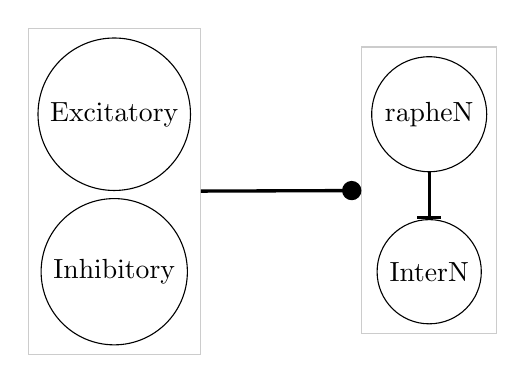
\begin{tikzpicture}[scale=1 
        , node distance = 2cm
        , every node/.style={  } 
        ]
        \node[draw,circle] (exc) at (0,0) {Excitatory};
        \node (inhb) [draw,circle,below of=exc] {Inhibitory};
        \node (lhb) [draw=black!20,fit={(exc) (inhb)}] {};

        \node (interneurons) [draw,circle,right of=exc,xshift=2cm]  {rapheN};
        \node (rNeuron) [draw,circle,below of=interneurons] {InterN};
        \node (raphe) [draw=black!20, fit={(rNeuron) (interneurons)}] {};

        \draw[-|,very thick] (interneurons) -- (rNeuron);
        \draw[-*,very thick] (lhb) -- (raphe);



    \end{tikzpicture}    

\end{figure}

\end{document}
